% Created by tikzDevice version 0.12.6 on 2026-02-22 21:43:40
% !TEX encoding = UTF-8 Unicode
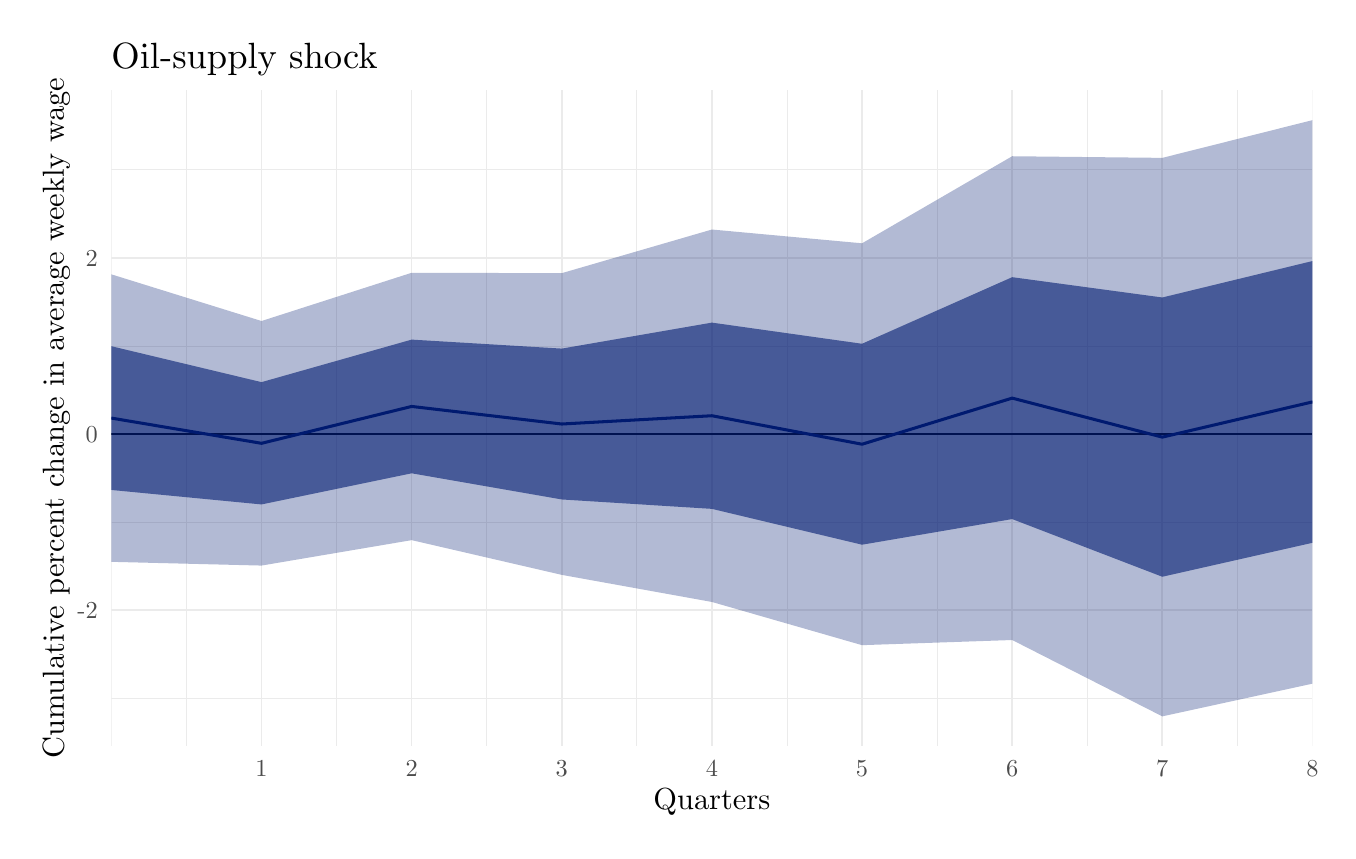
\begin{tikzpicture}[x=1pt,y=1pt]
\definecolor{fillColor}{RGB}{255,255,255}
\path[use as bounding box,fill=fillColor,fill opacity=0.00] (0,0) rectangle (469.75,290.32);
\begin{scope}
\path[clip] ( 30.25, 30.69) rectangle (464.26,267.67);
\definecolor{drawColor}{gray}{0.92}

\path[draw=drawColor,line width= 0.3pt,line join=round] ( 30.25, 47.99) --
	(464.26, 47.99);

\path[draw=drawColor,line width= 0.3pt,line join=round] ( 30.25,111.65) --
	(464.26,111.65);

\path[draw=drawColor,line width= 0.3pt,line join=round] ( 30.25,175.31) --
	(464.26,175.31);

\path[draw=drawColor,line width= 0.3pt,line join=round] ( 30.25,238.96) --
	(464.26,238.96);

\path[draw=drawColor,line width= 0.3pt,line join=round] ( 30.25, 30.69) --
	( 30.25,267.67);

\path[draw=drawColor,line width= 0.3pt,line join=round] ( 57.37, 30.69) --
	( 57.37,267.67);

\path[draw=drawColor,line width= 0.3pt,line join=round] (111.62, 30.69) --
	(111.62,267.67);

\path[draw=drawColor,line width= 0.3pt,line join=round] (165.87, 30.69) --
	(165.87,267.67);

\path[draw=drawColor,line width= 0.3pt,line join=round] (220.12, 30.69) --
	(220.12,267.67);

\path[draw=drawColor,line width= 0.3pt,line join=round] (274.38, 30.69) --
	(274.38,267.67);

\path[draw=drawColor,line width= 0.3pt,line join=round] (328.63, 30.69) --
	(328.63,267.67);

\path[draw=drawColor,line width= 0.3pt,line join=round] (382.88, 30.69) --
	(382.88,267.67);

\path[draw=drawColor,line width= 0.3pt,line join=round] (437.13, 30.69) --
	(437.13,267.67);

\path[draw=drawColor,line width= 0.6pt,line join=round] ( 30.25, 79.82) --
	(464.26, 79.82);

\path[draw=drawColor,line width= 0.6pt,line join=round] ( 30.25,143.48) --
	(464.26,143.48);

\path[draw=drawColor,line width= 0.6pt,line join=round] ( 30.25,207.13) --
	(464.26,207.13);

\path[draw=drawColor,line width= 0.6pt,line join=round] ( 84.50, 30.69) --
	( 84.50,267.67);

\path[draw=drawColor,line width= 0.6pt,line join=round] (138.75, 30.69) --
	(138.75,267.67);

\path[draw=drawColor,line width= 0.6pt,line join=round] (193.00, 30.69) --
	(193.00,267.67);

\path[draw=drawColor,line width= 0.6pt,line join=round] (247.25, 30.69) --
	(247.25,267.67);

\path[draw=drawColor,line width= 0.6pt,line join=round] (301.50, 30.69) --
	(301.50,267.67);

\path[draw=drawColor,line width= 0.6pt,line join=round] (355.75, 30.69) --
	(355.75,267.67);

\path[draw=drawColor,line width= 0.6pt,line join=round] (410.00, 30.69) --
	(410.00,267.67);

\path[draw=drawColor,line width= 0.6pt,line join=round] (464.26, 30.69) --
	(464.26,267.67);
\definecolor{drawColor}{RGB}{0,0,0}

\path[draw=drawColor,line width= 0.6pt,line join=round] ( 30.25,143.48) -- (464.26,143.48);
\definecolor{drawColor}{RGB}{0,26,112}

\path[draw=drawColor,line width= 1.1pt,line join=round] ( 30.25,149.24) --
	( 84.50,140.13) --
	(138.75,153.45) --
	(193.00,147.10) --
	(247.25,150.09) --
	(301.50,139.80) --
	(355.75,156.46) --
	(410.00,142.36) --
	(464.26,155.09);
\definecolor{fillColor}{RGB}{0,26,112}

\path[fill=fillColor,fill opacity=0.60] ( 30.25,175.21) --
	( 84.50,162.23) --
	(138.75,177.60) --
	(193.00,174.35) --
	(247.25,183.74) --
	(301.50,176.10) --
	(355.75,200.16) --
	(410.00,192.82) --
	(464.26,205.99) --
	(464.26,104.18) --
	(410.00, 91.91) --
	(355.75,112.75) --
	(301.50,103.49) --
	(247.25,116.44) --
	(193.00,119.84) --
	(138.75,129.29) --
	( 84.50,118.04) --
	( 30.25,123.27) --
	cycle;

\path[] ( 30.25,175.21) --
	( 84.50,162.23) --
	(138.75,177.60) --
	(193.00,174.35) --
	(247.25,183.74) --
	(301.50,176.10) --
	(355.75,200.16) --
	(410.00,192.82) --
	(464.26,205.99);

\path[] (464.26,104.18) --
	(410.00, 91.91) --
	(355.75,112.75) --
	(301.50,103.49) --
	(247.25,116.44) --
	(193.00,119.84) --
	(138.75,129.29) --
	( 84.50,118.04) --
	( 30.25,123.27);
\definecolor{fillColor}{RGB}{0,26,112}

\path[fill=fillColor,fill opacity=0.30] ( 30.25,201.18) --
	( 84.50,184.32) --
	(138.75,201.75) --
	(193.00,201.61) --
	(247.25,217.38) --
	(301.50,212.40) --
	(355.75,243.86) --
	(410.00,243.27) --
	(464.26,256.90) --
	(464.26, 53.28) --
	(410.00, 41.46) --
	(355.75, 69.05) --
	(301.50, 67.19) --
	(247.25, 82.80) --
	(193.00, 92.59) --
	(138.75,105.14) --
	( 84.50, 95.95) --
	( 30.25, 97.30) --
	cycle;

\path[] ( 30.25,201.18) --
	( 84.50,184.32) --
	(138.75,201.75) --
	(193.00,201.61) --
	(247.25,217.38) --
	(301.50,212.40) --
	(355.75,243.86) --
	(410.00,243.27) --
	(464.26,256.90);

\path[] (464.26, 53.28) --
	(410.00, 41.46) --
	(355.75, 69.05) --
	(301.50, 67.19) --
	(247.25, 82.80) --
	(193.00, 92.59) --
	(138.75,105.14) --
	( 84.50, 95.95) --
	( 30.25, 97.30);
\end{scope}
\begin{scope}
\path[clip] (  0.00,  0.00) rectangle (469.75,290.32);
\definecolor{drawColor}{gray}{0.30}

\node[text=drawColor,anchor=base east,inner sep=0pt, outer sep=0pt, scale=  0.88] at ( 25.30, 76.79) {-2};

\node[text=drawColor,anchor=base east,inner sep=0pt, outer sep=0pt, scale=  0.88] at ( 25.30,140.45) {0};

\node[text=drawColor,anchor=base east,inner sep=0pt, outer sep=0pt, scale=  0.88] at ( 25.30,204.10) {2};
\end{scope}
\begin{scope}
\path[clip] (  0.00,  0.00) rectangle (469.75,290.32);
\definecolor{drawColor}{gray}{0.30}

\node[text=drawColor,anchor=base,inner sep=0pt, outer sep=0pt, scale=  0.88] at ( 84.50, 19.68) {1};

\node[text=drawColor,anchor=base,inner sep=0pt, outer sep=0pt, scale=  0.88] at (138.75, 19.68) {2};

\node[text=drawColor,anchor=base,inner sep=0pt, outer sep=0pt, scale=  0.88] at (193.00, 19.68) {3};

\node[text=drawColor,anchor=base,inner sep=0pt, outer sep=0pt, scale=  0.88] at (247.25, 19.68) {4};

\node[text=drawColor,anchor=base,inner sep=0pt, outer sep=0pt, scale=  0.88] at (301.50, 19.68) {5};

\node[text=drawColor,anchor=base,inner sep=0pt, outer sep=0pt, scale=  0.88] at (355.75, 19.68) {6};

\node[text=drawColor,anchor=base,inner sep=0pt, outer sep=0pt, scale=  0.88] at (410.00, 19.68) {7};

\node[text=drawColor,anchor=base,inner sep=0pt, outer sep=0pt, scale=  0.88] at (464.26, 19.68) {8};
\end{scope}
\begin{scope}
\path[clip] (  0.00,  0.00) rectangle (469.75,290.32);
\definecolor{drawColor}{RGB}{0,0,0}

\node[text=drawColor,anchor=base,inner sep=0pt, outer sep=0pt, scale=  1.10] at (247.25,  7.64) {Quarters};
\end{scope}
\begin{scope}
\path[clip] (  0.00,  0.00) rectangle (469.75,290.32);
\definecolor{drawColor}{RGB}{0,0,0}

\node[text=drawColor,rotate= 90.00,anchor=base,inner sep=0pt, outer sep=0pt, scale=  1.10] at ( 13.08,149.18) {Cumulative percent change in average weekly wage};
\end{scope}
\begin{scope}
\path[clip] (  0.00,  0.00) rectangle (469.75,290.32);
\definecolor{drawColor}{RGB}{0,0,0}

\node[text=drawColor,anchor=base west,inner sep=0pt, outer sep=0pt, scale=  1.32] at ( 30.25,275.73) {Oil-supply shock};
\end{scope}
\end{tikzpicture}
